% !TEX root=/home/tavant/these/manuscript/src/manuscript.tex

\section{Canonical simulation results}
  \label{sec-canonical}
  
  
  The {\it canonical} case corresponds to the case when the wall do not include its dielectric mechanism:
  \begin{itemize}
    \item the dielectric layer on the plasma potential
    \item the electron emission
  \end{itemize}
  It is the reference case that will be extensively described and commented.
  It will be used then to analyse and quantify the effects of the two aspects of the dielectric walls.
  
  \subsection{Initial phase} \label{subsec-initlaphase}
  The initial phase of the simulation corresponds to the growth of the \ac{ECDI}, and the formation of the sheaths.
  Because of growth of the instability, the electron transport increases as well, that increases the electron heating.
  
  The time scale of the sheath formation is governed by the ion inertia.
  It is roughly the same time scale than the saturation of the instability due to ion-trapping.
  
  \begin{figure}[hbtp]
    \centering
    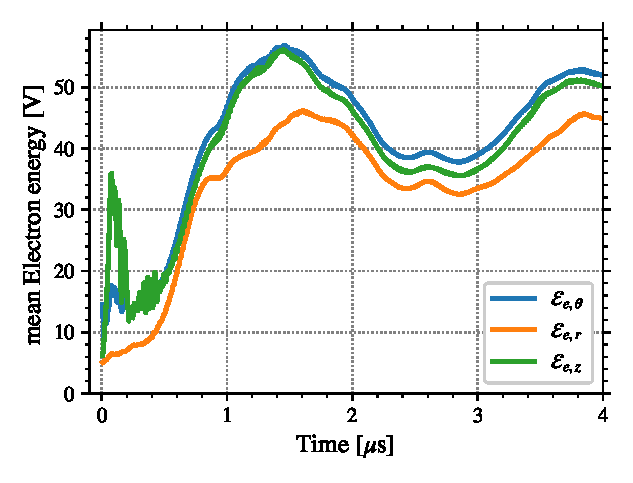
\includegraphics[width=\defaultwidth]{canonical_Te_start_directions}
    \caption{Temporal evolution of the electron mean kinetic energy decomposed over the three direction. Is showed only the beginning of the simulation.}
    \label{fig-canon_Te_strat}
  \end{figure}
  
  \Cref{fig-canon_Te_strat} shows the temporal evolution of the electron mean kinetic energy decomposed over the three direction, $\Ee_r, \Ee_{\theta}, \Ee_z$, such that
  \begin{equation} \label{eq-Ee_direction}
    \Ee_d = \frac{1}{n} \frac{1}{2} m_e \iiint_{\vect{v}}  v_{e,d}^2 f (\vect{v}) d^3v, \text{ with } d \in \{r, \theta, z  \}
  \end{equation}
  
  We see that after some high frequency oscillations of $\Ee_{\theta}$ and $\Ee_z$ due to the cyclotron motion, the temperature rises before Stabilizing at $\Ee \simeq 45$V.
  The radial temperature $\Te_r$ is less than $\Te_z$ and $\Te_{\theta}$, but only by a small factor.
  This means that the electrons temperature is quite anisotropic.
  
  \renewcommand\subfigurewidth{4in}
  
  \begin{figure}[hbtp]
    \centering
    \begin{tabular}{c}
      \subfigure{time_r_mean_n}{a}{20, 20}
          \\
      \subfigure{time_r_mean_phi}{b}{20, 20} 
    \end{tabular}
    \caption{Temporal evolution of the radial profile of the ({\bf a}) electron density and ({\bf b}) the plasma potential averaged azimuthally}
    \label{fig-tx_n_phi}
  \end{figure}

  We can see on \Cref{fig-tx_n_phi} the evolution of the radial profile of the electron density on the plasma potential on the same time scale.
  We observe of the two parameters the formation of the sheath and the evolution toward a steady state.
  
  \subsection{Stable phase} \label{subsec-stablephase}
  After the relatively fast rise of the plasma characteristic, the simulations stabilises at a steady state, as we can see in \Cref{fig-canon_Te_all}.
  
  We observe that after $t\simeq2\mus$ , the electron energy $\Ee$ start to oscillate around its final value.
  The oscillations are than damped and reach their minimum amplitude at  $t\simeq 7\mus$.
  Hence, there is no need to simulate for longer than $10\mus$ in the following simulations.
  
  \inlinenote{Je parle ici d'oscillation. Devrais-je en parler ? Peut-être plus tard ?}
  
  
  
  \begin{figure}[hbtp]
    \centering
    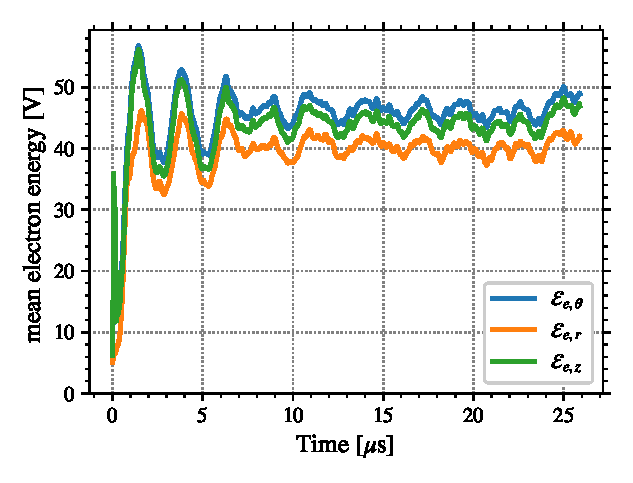
\includegraphics[width=\defaultwidth]{canonical_Te_all_directions}
    \caption{Temporal evolution of the electron mean kinetic energy decomposed over the three direction, similar to \cref{fig-canon_Te_strat} but during a longer time}
    \label{fig-canon_Te_all}
  \end{figure}
  

  \Cref{fig-profiles} shows the radial profiles of the electron and ions densities averaged azimuthally at steady state.
  We can see the sheath close to the wall where the electron density fall rapidly compare to the ions.
  
  \begin{figure}[hbtp]
    \centering
    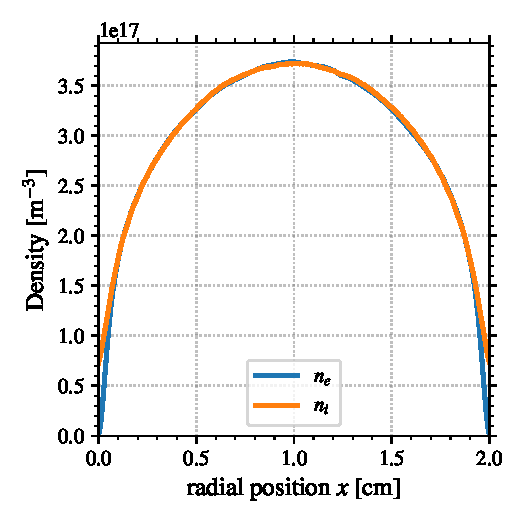
\includegraphics[width=\defaultwidth]{density_profile.pdf}
    \caption{Radial profile of the ion and electron densities at steady state, average azimuthally.}
    \label{fig-profiles}
  \end{figure}
  
  \subsection{Enhanced electron transport} \label{subsec-canonmue}
  The electron cross-field axial transport is usually characterized by the electron mobility
  \begin{equation} \label{eq-mobdef}
    \mob = \frac{u_{e, z}}{E_z}
  \end{equation}
  with $u_{e,z}$ and $E_z$ the electron mean axial velocity and the axial electric field, respectively./
  \nomenclature[Q]{\ensuremath{ \mob}}{ Electron mobility}
  \nomenclature[Q]{\ensuremath{ u}}{ Electron mean velocity}
  
  In the \ac{PIC} simulations, \mob is computed at each time step by
  \begin{equation} \label{eq-mobpic}
    \mobpic = \frac{1}{E_z} \sum_N v_{e,z}
  \end{equation}

  \begin{figure}[hbtp]
    \centering
    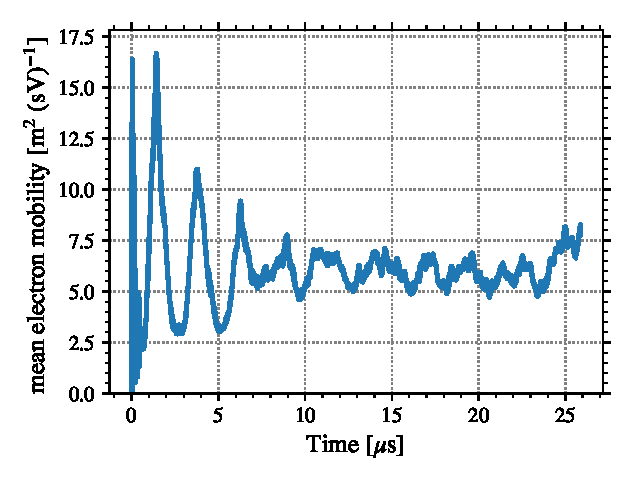
\includegraphics[width=\defaultwidth]{canonical_mu_all}
    \caption{Temporal evolution of the electron axial mobility computed in the \ac{PIC} simulation.}
    \label{fig-canon_mu}
  \end{figure}
  
  \Cref{fig-canon_mu} shows the temporal evolution of the electron mobility $\mobpic$ measured in the simulation.
  We can see that it presents the same characteristics that the evolution of the electron energy $\Ee$ on \cref{fig-canon_Te_all}.
  
  The classical electron mobility from the collisional theory is \citep{lafleur2016a}
  \begin{equation} \label{eq-muclass}
    \mobcla = \frac{\nu_m \frac{e}{m_e}}{\oce^2 + \nu_m^2}
  \end{equation}
  with $\nu_m$ the electron-neutral  collision frequency and \oce is the electron cyclotron frequency.
  In the conditions of \cref{parameters}, $\mobcla \simeq 0.8$ m$^2$(sV)$^{-1}$.
  
  The measured electron mobility in the \ac{PIC} simulation is one order of magnitude larger than the classical mobility.
  Is the present case, as no electron is emitted from the wall, the enhancement only comes from the \ac{ECDI}, as proposed by \citet{lafleur2016} .
  % K_ex = 2 10^-13
  % n_g = 1e19
  % wce = q B / m
  \Cref{fig-exampleECDI} illustrates the \ac{ECDI} by showing the azimuthal electric at the center of the channel.
  We can clearly see the oscillation pasterns, of wavelength of the order of 1~mm, as observed in \citet{heron2013,janhunen2018} [Other REFs needed !].
  The instability is the subject of Chapter 5 [Use REF here], hence it will not be further investigated.
  
  
  \begin{figure}[hbtp]
    \centering
    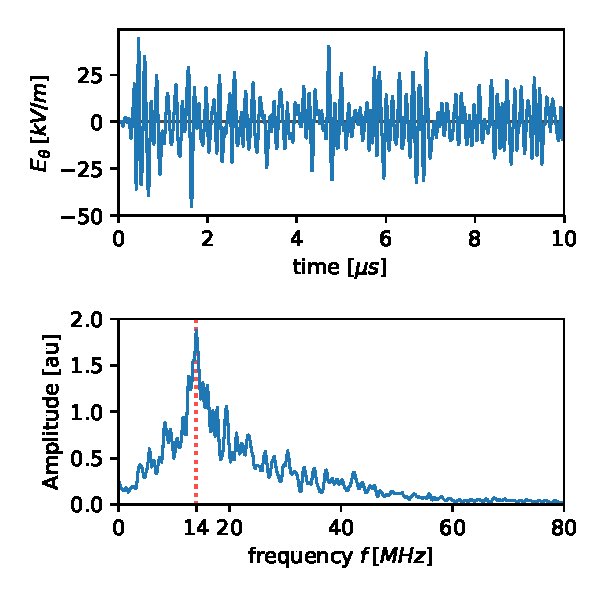
\includegraphics[width=\defaultwidth]{time_and_FFT}
    \caption{Azimuthal instability: temporal evolution of the azimuthal electric field at the center of the simulation, and its frequency spectra }
    \label{fig-exampleECDI}
  \end{figure}

  
  